\documentclass[15pt]{beamer} % [12pt]
%\documentclass[15pt,aspectratio=1610]{beamer} % [12pt]
%\documentclass[15pt,letterpaper,handout]{beamer} % [12pt]

%\usepackage{fontspec}
\usepackage[spanish]{babel}
\usepackage[utf8]{inputenc}
\usepackage{textcomp}
\usepackage{multicol}
\usepackage{tikz}
\usetikzlibrary{shapes.geometric, arrows, plotmarks}

\usepackage{pgfplots}

% For handout
%\usepackage{pgfpages}
%\pgfpagesuselayout{4 on 1}[letterpaper,landscape,border shrink=5mm]
% End of handout

\usetheme{Warsaw}
\expandafter\def\expandafter\insertshorttitle\expandafter{%
  \insertshorttitle\hfill%
  \insertframenumber\,/\,\inserttotalframenumber}

%\usetheme{PaloAlto}
%\usetheme{Marburg} % Barra azul a la derecha
%\usetheme{Madrid}

% What is this all about:
\title[Paralelización del filtro DNLM]{Implementación paralela de optimizaciones computacionales \\del
filtro DNLM para la plataforma Xeon Phi}
\subtitle{Trabajo Final de Graduaci\'on}
\institute[TEC]{Área Académica de Ingeniería en Computadores \\ Tecnológico de Costa Rica}
\date[Junio 2018]{11 Junio, 2018}
\author[M.\ Zumbado]{Ing.\ Manuel Zumbado Corrales}

%%%%%%%%%%%%%%%%%%%%%%%%%%%%%%%%%%%%%%%%%%%%%%%%%%%%%%%%%%%%%%%%%%%%%%%%%%%%
%  Notación

\usepackage{mathrsfs}                   % Calygraphic fonts for transforms

\renewcommand{\Re}{\operatorname{Re}}
\renewcommand{\Im}{\operatorname{Im}}

\newcommand{\prt}[1]{\ensuremath{\mathcal{#1}}}         %% partitioning
\newcommand{\img}[1]{\ensuremath{\mathcal{#1}}}         %% image as a set
\newcommand{\reg}[1][R]{\ensuremath{\mathcal{#1}}}      %% region
\newcommand{\pred}[1]{\ensuremath{\mathrm{#1}}}         %% predicate
\newcommand{\operat}[2]{\mathcal{#1}\left\{#2\right\}}
\newcommand{\transf}[1]{\mathscr{#1}}
\newcommand{\fourier}[1]{\transf{F}\left\{#1\right\}}
\newcommand{\ifourier}[1]{\transf{F}^{-1}\left\{#1\right\}}
\newcommand{\laplace}[1]{\transf{L}\left\{#1\right\}}
\newcommand{\ulaplace}[1]{\transf{L}_u\left\{#1\right\}}
\newcommand{\blaplace}[1]{\transf{L}_b\left\{#1\right\}}
\newcommand{\ilaplace}[1]{\transf{L}^{-1}\left\{#1\right\}}
\newcommand{\ztrans}[1]{\transf{Z}\left\{#1\right\}}
\newcommand{\iztrans}[1]{\transf{Z}^{-1}\left\{#1\right\}}
\newcommand{\zutrans}[1]{\transf{Z}_u\left\{#1\right\}}
\newcommand{\exceq}{\ensuremath{\overset{!}{=}}}

\newcommand{\signum}{\operatorname{signum}}
\newcommand{\pos}{\operatorname{pos}}
\newcommand{\val}{\operatorname{val}}
\newcommand{\vct}[1]{\ensuremath{\underline{\mathbf{#1}}}}
\newcommand{\pix}[1]{\ensuremath{\mathbf{#1}}}
\newcommand{\mat}[1]{\ensuremath{\mathbf{#1}}}
\newcommand{\vctmu}{\vct{\boldsymbol{\mu}}}
\newcommand{\vctzeta}{\vct{\boldsymbol{\zeta}}}
\newcommand{\vctpi}{\vct{\boldsymbol{\pi}}}
\newcommand{\vctvarphi}{\vct{\boldsymbol{\varphi}}}
\newcommand{\raum}[1]{\ensuremath{\mathbb{#1}}}
\newcommand{\matSigma}{\mat{\boldsymbol{\Sigma}}}
\newcommand{\matLambda}{\mat{\boldsymbol{\Lambda}}}
\newcommand{\matPsi}{\mat{\boldsymbol{\Psi}}}
\newcommand{\matPhi}{\mat{\boldsymbol{\Phi}}}
\newcommand{\row}[2]{\ensuremath{\mathbf{\underline{#1}_{#2(\cdot)}}}}
\newcommand{\col}[2]{\ensuremath{\mathbf{\underline{#1}_{(\cdot) #2}}}}
\newcommand{\seq}[1]{\ensuremath{#1}}
\newcommand{\set}[1]{\ensuremath{\mathcal{#1}}}
\newcommand{\gset}[1]{\ensuremath{#1}} %% set for greek symbols
\newcommand{\front}[1]{\widehat{\set{#1}}}
\newcommand{\setlambda}{\set{\boldsymbol{\lambda}}}
\newcommand{\klass}[1]{\ensuremath{\mathpss{#1}}}
\newcommand{\graph}[1]{\ensuremath{\mathsf{#1}}}
\newcommand{\lab}[1]{\ensuremath{\mathpss{L}(#1)}}
\newcommand{\myfrac}[2]{{\footnotesize #1/#2}}
\newcommand{\ifthenspc}{\rule{3mm}{0mm}}
\newcommand{\point}[1]{\ensuremath{\mathsf{#1}}}
\newcommand{\estim}[1]{\ensuremath{\hat{#1}}}
\newcommand{\numset}[1]{\ensuremath{\mathbb{#1}}}
\newcommand{\tuple}[1]{\ensuremath{\left\langle#1\right\rangle}}
\newcommand{\conj}[1]{\ensuremath{{{#1}^{\ast}}}}
\newcommand{\base}[1]{\set{#1}}
\newcommand{\zeron}[1]{\ensuremath{\underset{\uparrow}{#1}}}
\newcommand{\sysT}{\ensuremath{\mathcal{T}}}
\newcommand{\sys}[1]{\ensuremath{\sysT\left[#1\right]}}
\newcommand{\sen}{\operatorname{sen}} % sinus in spanish (seno)
\newcommand{\senh}{\operatorname{senh}} % sinus hiperbolicus in spanish (seno)
\newcommand{\arcsen}{\operatorname{arcsen}} % arcus sinus hiperbolicus in spanish (arcoseno)
\newcommand{\sgn}{\operatorname{sgn}} % signus
\newcommand{\roc}{\text{ROC: }}

\newcommand{\code}[1]{\texttt{#1}}
\newcommand{\conv}{\ensuremath{\ast}}
\newcommand{\cconv}{\ensuremath{\;\,\text{\footnotesize{N}}\!\!\!\!\!\!\bigcirc}}
\newcommand{\Ln}{\operatorname{Ln}}
\newcommand{\sa}{\operatorname{sa}}
\newcommand{\senc}{\operatorname{senc}}
\newcommand{\si}{\operatorname{si}}

%% Natural, Integer and Real Numbers
\newcommand{\setA}{\ensuremath{\mathbb{A}}}
\newcommand{\setB}{\ensuremath{\mathrm{I\negthinspace B}}}
\newcommand{\setC}{\ensuremath{\mathbb{C}}}
\newcommand{\setD}{\ensuremath{\mathrm{I\negthinspace D}}}
\newcommand{\setE}{\ensuremath{\mathrm{I\negthinspace E}}}
\newcommand{\setF}{\ensuremath{\mathrm{I\negthinspace F}}}
\newcommand{\setG}{\ensuremath{\mathbb{G}}}
\newcommand{\setH}{\ensuremath{\mathrm{I\negthinspace H}}}
\newcommand{\setI}{\ensuremath{\mathbb{I}}}
\newcommand{\setJ}{\ensuremath{\mathbb{J}}}
\newcommand{\setK}{\ensuremath{\mathrm{I\negthinspace K}}}
\newcommand{\setL}{\ensuremath{\mathrm{I\negthinspace L}}}
\newcommand{\setM}{\ensuremath{\mathrm{I\negthinspace M}}}
\newcommand{\setN}{\ensuremath{\mathrm{I\negthinspace N}}}
\newcommand{\setO}{\ensuremath{\mathbb{O}}}
\newcommand{\setP}{\ensuremath{\mathrm{I\negthinspace P}}}
\newcommand{\setQ}{\ensuremath{\mathbb{Q}}}
\newcommand{\setR}{\ensuremath{\mathrm{I\negthinspace R}}}
\newcommand{\setS}{\ensuremath{\mathbb{S}}}
\newcommand{\setT}{\ensuremath{\mathbb{T}}}
\newcommand{\setU}{\ensuremath{\mathbb{U}}}
\newcommand{\setV}{\ensuremath{\mathbb{V}}}
\newcommand{\setW}{\ensuremath{\mathbb{W}}}
\newcommand{\setX}{\ensuremath{\mathbb{X}}}
\newcommand{\setY}{\ensuremath{\mathbb{Y}}}
\newcommand{\setZ}{\ensuremath{\mathbb{Z}}}


\tikzstyle{startstop} = [rectangle, rounded corners, minimum width=3cm, minimum height=1cm,text centered, draw=black]
\tikzstyle{io} = [trapezium, trapezium left angle=70, trapezium right angle=110, minimum width=3cm, minimum height=1cm, text centered, draw=black]
\tikzstyle{process} = [rectangle, minimum width=3cm, minimum height=1cm, text centered, text width=3cm, draw=black]
\tikzstyle{decision} = [diamond, minimum width=3cm, minimum height=1cm, text centered, draw=black]
\tikzstyle{arrow} = [thick,->,>=stealth]

%%%%%%%%%%%%%%%%%%%%%%%%%%%%%%%%%%%%%%%%%%%%%%%%%%%%%%%%%%%%%%%%%%%%%%%%%%%%

\begin{document}
\graphicspath{{./}{./fig/}}

\begin{frame}
  \titlepage
\end{frame}


\begin{frame}{Contenido}
  \tableofcontents
\end{frame}

% Título para el contexto
\section{Preprocesamiento de videos de actividad celular}

\begin{frame}{Contexto}
  
  \begin{itemize}
      \item Proyecto FEES ‘‘Análisis funcional genómico de células cancerosas por RNA de interferencia para la identificación de redes de regulación asociadas a proliferación y muerte en respuesta a quimioterapia genotóxica’’
      \item Participan laboratorios de investigación del TEC, UCR y CeNAT
  \end{itemize}
\end{frame}


\begin{frame}{Contexto}

\begin{columns}
    \column{.45\textwidth}
    \begin{enumerate}
    \item <1-| alert@1> Imagen de entrada
    \item <2-| alert@2> Ecualizaci\'on de histogramas CLAHE
    \item <3-| alert@3> Filtro DNLM
    \item <4-| alert@4> Segmentaci\'on
    \end{enumerate}
    \column{.5\textwidth}
    \only<1>{\includegraphics[width=0.9\textwidth]{BBBC006_original}}     
    \only<2>{\includegraphics[width=0.9\textwidth]{BBBC006_clahe}}  
    \only<3>{\includegraphics[width=0.9\textwidth]{BBBC006_preprocessed}}
    \only<4>{\includegraphics[width=0.9\textwidth]{BBBC006_segmented}}
  \end{columns}
\end{frame}

\begin{frame}{Flujo de procesamiento para videos de actividad celular}
\begin{center}
\only<1>{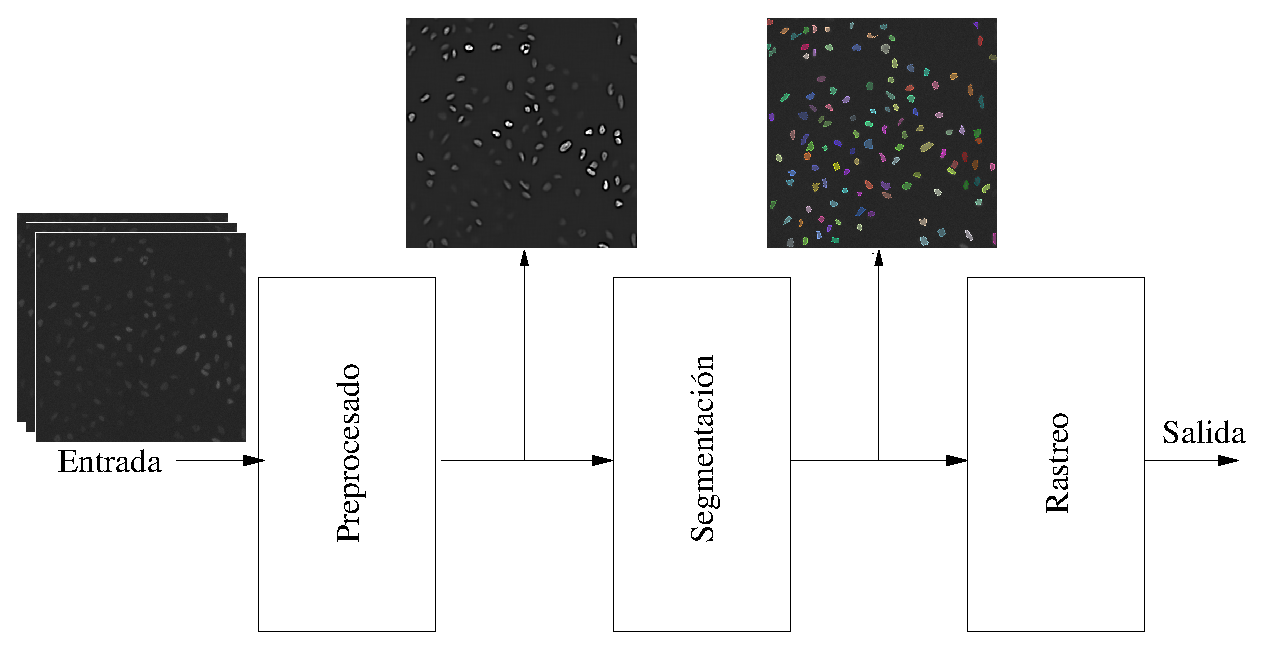
\includegraphics[width=0.9\linewidth]{diagram}}     
\only<2>{\includegraphics[width=0.9\linewidth]{diagram_high}}  
\end{center}
\end{frame}

\begin{frame}{Problema}
  
  \begin{itemize}
  \item Complejidad computacional del filtro DNLM
  \item Se requieren preprocesar lotes de hasta 170000 im\'agenes
  \end{itemize}
\end{frame}

\begin{frame}{Objetivos}
  \begin{itemize}
  \item Proponer una optimización computacional y paralelización del filtro DNLM  para la plataforma \textit{Xeon Phi Knights Landing}
  \vspace{3mm}
  \item Paralelismo en dos niveles: a nivel de tareas y a nivel del datos
  \vspace{3mm}
  \item Evaluar el rendimiento de las dos optimizaciones computacionales paralelas 
  \end{itemize}
\end{frame}



\section{Solución}



\begin{frame}
	Implementaci\'on paralela de tres algoritmos:
	\begin{itemize}
	\item DNLM: Filtro \textit{Deceived Non Local Means} original
	\item DNLM-IIFFT: Filtro \textit{Deceived Non Local Means} con Im\'agenes Integrales y FFT
	\item DNLM-MA: Filtro \textit{Deceived Non Local Means} con Media movil y simetr\'ia
	\end{itemize}
	
	Complejidad computacional para una imagen de entrada de $N$ pixeles, ventana de b\'usqueda de $S$ pixeles y tama\~no de vecindario de $W$ pixeles:
	\begin{itemize}
	\item DNLM: $\mathcal{O}(N\cdot S\cdot W)$ 
	\item DNLM-IIFFT: $\mathcal{O}(N \cdot S\log S)$
	\item DNLM-MA: $\mathcal{O}(N\cdot S\cdot \sqrt{W})$
	\end{itemize}

\end{frame}



\section{Experimento}

\begin{frame}{Métricas utilizadas}
	\begin{itemize}
		\item $\text{CPI}_{\text{hilo}} = \frac{\text{\# de ticks de reloj}}{\# \text{de instrucciones}}$
		\vspace*{4mm}
		\item $\text{CPI}_{\text{CPU}} = \frac{\text{CPI}_{\text{hilo}}}{\text{cantidad CPU}}$
		\vspace*{4mm}
		\item $\text{VPU}_{\text{i}}= \frac{\text{\# SIMD empaquetadas}}{\text{\# SIMD empaquetadas}+\text{\# SIMD escalares}}$
	\end{itemize}	
\end{frame}
	
	
	
\begin{frame}{Métricas utilizadas}
	\begin{itemize}
	\item $\mu\text{Ops}_{\text{i}}= \frac{\text{\#}\mu\text{Ops retiradas MS}}{\text{\#}\mu\text{Ops retiradas totales}}$
	\vspace*{4mm}
	\item $\text{L1}_{\text{Hit}} = \frac{\text{\# operaciones de lectura}-\text{\# fallos de lectura en L1}}{\text{\# operaciones de lectura}}$
	\vspace*{4mm}
	\item $\text{L2}_{\text{Hit}} = \frac{\text{\# operaciones de lectura}-\text{\# fallos de lectura en L2}}{\text{\# operaciones de lectura}}$
	\end{itemize}
\end{frame}
	
	

\begin{frame}{Experimento}

Configuración:
	\begin{itemize}
		\item Promedio de 10 ejecuciones por prueba
		\item Imagen de entrada de $N = 1024\times 1024$ pixeles, con $S = 21\times21$ y $W = 7\times7$
		\item Se escala la cantidad de hilos de 1 a 256
	\end{itemize}
	
	

\end{frame}

\section{Resultados}


\begin{frame}{Escalabilidad de optimizaciones del filtro DNLM}

	\begin{center}
		\begin{tikzpicture}
      \begin{semilogyaxis}[
          height=0.9\textheight,
          width=0.9\textwidth,
          xlabel= N\'umero de hilos,
          ylabel=Duraci\'on (s),
          xmin=1,
          xmax=260,
          scaled x ticks = false
  ]
           \addplot[mark=*] table[x=Threads,y=Time] {data/scaling_original.txt};
           \addlegendentry{DNLM}
          \addplot[mark=x] table[x=Threads,y=Time] {data/scaling_iifft.txt};
          \addlegendentry{DNLM-IIFFT-P}
          \addplot[mark=triangle] table[x=Threads,y=Time] {data/scaling_condat.txt};
          \addlegendentry{DNLM-MA-P}
      \end{semilogyaxis}
  \end{tikzpicture}
	\end{center}
\end{frame}


\begin{frame}{Eficiencia de las implementaciones paralelas del filtro DNLM}

	\begin{center}
		\begin{tikzpicture}
      \begin{axis}[
          height=0.8\textheight,
          width=0.8\textwidth,
          xlabel= N\'umero de hilos,
          ylabel=Eficiencia,
          xmin=1,
          xmax=260,
          %scaled x ticks = false
  ]
           \addplot[mark=*] table[x=Threads,y=Efficiency] {data/eficiency_original.txt};
           \addlegendentry{DNLM-P}
          \addplot[mark=x] table[x=Threads,y=Efficiency] {data/eficiency_iifft.txt};
          \addlegendentry{DNLM-IIFFT-P}
          \addplot[mark=triangle] table[x=Threads,y=Efficiency] {data/efficiency_condat.txt};
          \addlegendentry{DNLM-MA-P}
      \end{axis}     
  \end{tikzpicture}
	\end{center}
\end{frame}

\begin{frame}{Aceleraci\'on alcanzada con las optimizaciones del filtro DNLM}
  


  \begin{center}
    {\footnotesize Aceleración promedio de optimizaciones del filtro DNLM}
    \begin{tabular}{lrrr}
	Filtro & Duración [s]& Coef. de var. & Aceleración [$\times$]\tabularnewline
	\hline
	DNLM & $163,71\pm1,32$ & $0,01$ & $1$\tabularnewline
	DNLM-IIFFT & $76,68\pm0,06$ & $0,00$ & $2,14$\tabularnewline
	DNLM-MA & $1,81\pm 0,01$ & $0,00$ & $90,44$ \tabularnewline
	DNLM-P & $1,5\pm0,10$ & $0,06$ & $108,99$\tabularnewline
	DNLM-IIFFT-P & $1,00\pm0,00$ & $0,00$ & $163,92$ \tabularnewline 
	DNLM-MA-P & $\boldsymbol{0,25\pm0,00}$ & $\boldsymbol{0,01}$ &  $\boldsymbol{665,63}$\tabularnewline
	\end{tabular}
  \end{center}
\end{frame}


\begin{frame}{Intensidad de uso de VPU}
  
  \begin{center}
    {\footnotesize Intensidad vectorial de operaciones con un hilo de ejecución}
    \begin{tabular}{lr}
	 Filtro & $\text{VPU}_{\text{i}}$ \tabularnewline
	\hline
	DNLM-P & 1,00 \tabularnewline
	DNLM-IIFFT-P & 0,81 \tabularnewline
	DNLM-MA-P & 0,95 \tabularnewline
	\end{tabular}
  \end{center}
\end{frame}


\begin{frame}{Ciclos por instrucción por núcleo}
  
  \begin{center}
   \setlength\tabcolsep{2.5pt}
   \setlength{\textfloatsep}{25mm}
    {\footnotesize Cambio en $\text{CPI}_{\text{CPU}}$ al escalar el n\'umero de hilos}
    \begin{tabular}{lrrrrrrrrr}
	 Filtro & 1 & 2 & 4 & 8 & 16 & 32 & 64 & 128 & 256 \tabularnewline
	\hline
	DNLM-P & 1,87 & 0,94 & 0,47 & 0,23 & 0,12 & 0,06 & 0,03 & 0,02 & 0,02 \tabularnewline
	DNLM-IIFFT-P & 1,36 & 0,68 & 0,34 & 0,17 & 0,09 & 0,04 & 0,02 & 0,02 & 0,02 \tabularnewline
	DNLM-MA-P & 1,74 & 1,03 & 0,54 & 0,27 & 0,14 & 0,07 & 0,04 & 0,02 & 0,02 \tabularnewline
	\end{tabular}
  \end{center}
\end{frame}

\begin{frame}{Intensidad de operaciones de microarquitectura}
  
  \begin{center}
  \setlength\tabcolsep{2.5pt}
   \setlength{\textfloatsep}{25mm}
    {\footnotesize Cambio en intensidad de  micro-operaciones al escalar el n\'umero de hilos}
    \begin{tabular}{lrrrrrrrrr}
	 Filtro & 1 & 2 & 4 & 8 & 16 & 32 & 64 & 128 & 256 \tabularnewline
	\hline
	DNLM-P & 0,26 & 0,26 & 0,26 & 0,26 & 0,26 & 0,27 & 0,27 & 0,27 & 0,28 \tabularnewline
	DNLM-IIFFT-P & 0,05 & 0,05 & 0,05 & 0,05 & 0,06 & 0,07 & 0,09 & 0,11 & 0,21 \tabularnewline
	DNLM-MA-P & 0,03 & 0,06 & 0,10 & 0,16 & 0,23 & 0,28 & 0,32 & 0,32 & 0,33 \tabularnewline
	\end{tabular}
  \end{center}
\end{frame}


\begin{frame}{Raz\'on de aciertos de lectura en cach\'e L1}
  
  \begin{center}
  \setlength\tabcolsep{2.5pt}
   \setlength{\textfloatsep}{25mm}
    {\footnotesize Cambio en la raz\'on de aciertos de lectura en cach\'e L1 al escalar el n\'umero de hilos}
    \begin{tabular}{lrrrrrrrrr}
	 Filtro & 1 & 2 & 4 & 8 & 16 & 32 & 64 & 128 & 256 \tabularnewline
	\hline
	DNLM-P & 0,99 & 0,99 & 1,00 & 1,00 & 1,00 & 1,00 & 1,00 & 0,99 & 0,99 \tabularnewline
	DNLM-IIFFT-P & 0,99 & 0,99 & 0,99 & 0,99 & 0,99 & 0,99 & 0,99 & 0,99 & 0,99 \tabularnewline
	DNLM-MA-P & 0,80 & 0,83 & 0,85 & 0,88 & 0,93 & 0,96 & 0,98 & 0,99 & 0,99 \tabularnewline
	\end{tabular}
  \end{center}
\end{frame}


\begin{frame}{Raz\'on de aciertos de lectura en cach\'e L2}
  
  \begin{center}
  \setlength\tabcolsep{2.5pt}
   \setlength{\textfloatsep}{25mm}
    {\footnotesize Cambio en la raz\'on de aciertos de lectura en cach\'e L2 al escalar el n\'umero de hilos}
    \begin{tabular}{lrrrrrrrrr}
	 Filtro & 1 & 2 & 4 & 8 & 16 & 32 & 64 & 128 & 256 \tabularnewline
	\hline
	DNLM-P & 0,99 & 0,99 & 0,97 & 0,96 & 0,96 & 0,95 & 0,94 & 0,97 & 0,95 \tabularnewline
	DNLM-IIFFT-P & 1,00 & 1,00 & 0,99 & 0,99 & 0,99 & 0,99 & 0,99 & 0,98 & 0,93 \tabularnewline
	DNLM-MA-P & 0,91 & 0,86 & 0,85 & 0,85 & 0,85 & 0,85 & 0,85 & 0,88 & 0,89 \tabularnewline
	\end{tabular}
  \end{center}
\end{frame}




\begin{frame}{Conclusiones}
  
  \begin{itemize}
  \item Se desarrollaron dos optimizaciones computacionales del filtro DNLM y sus paralelizaciones
  \item Se alcanz\'o un grado de vectorizaci\'on de 81\% para IIFFT, 95\% para MA y 100\% para el filtro original
  \item La escalabilidad de los algoritmos implementados se ve afectada por el ancho de banda de memoria y aciertos en cach\'e L2
  \item La mayor aceleraci\'on alcanzada ($1663\times$) supera la mejor aceleraci\'on reportada en el estado del arte ($740\times$)
  \item Procesamiento de un conjunto de 170000 im\'agenes en unas 11 horas
  \item Efectiva vectorizaci\'on es la clave en el escalamiento
  \item Eficiencia en tiempo de procesamiento permitir\'ia su uso en CNNs
  \item Art\'iculos relacionados publicados en CIARP 2017 y pr\'oximamente ICIP 2018
  \end{itemize}
  
\end{frame}

\begin{frame}{Trabajo futuro}
  
  \begin{itemize}
  \item Explorar paralelizaci\'on multi nodo 
  \item A\~nadir \textit{Unsharp Masking} adaptativo
  \item Calibraci\'on automática de par\'ametros
  \end{itemize}
  
\end{frame}


\section{Resumen}

\begin{frame}{Resumen}
  \tableofcontents
\end{frame}

\end{document}


